\documentclass{llncs}

\usepackage{amsmath}
\usepackage{graphicx}
\usepackage{url}
\usepackage{booktabs}

% llncs's default geometry targets Springer's small print trim size; this
% report is read as a PDF, so we use standard A4 margins instead. Loaded
% after \documentclass so it overrides the class's own settings.
\usepackage[a4paper, margin=2.3cm]{geometry}

\begin{document}

\title{Performance Analysis of Apache ZooKeeper's Write Pipeline\\
\large Software Performance Engineering --- Project Stage I}

\author{Gil Jorge (110062) \and Jo\~{a}o Palma (<STUDENT\_NUMBER>) \and
  Gabriel Petti Tavares (1120691)}

\institute{Instituto Superior T\'{e}cnico, Universidade de Lisboa\\
  Group 18}

\maketitle

\begin{abstract}
We evaluate the scalability of Apache ZooKeeper 3.9's write pipeline on
ensembles of 1, 3 and 5 servers by fitting Gunther's Universal
Scalability Law (USL) to a mixed read/write concurrency sweep (30\% writes,
1--80 clients). The load is generated by a multi-threaded Java client that
connects to every server in the ensemble. The fits ($R^2\ge0.99$) show a
contention coefficient $\alpha\approx0.22$--$0.24$ at every ensemble size
and a coherency coefficient $\beta\approx6$--$7\times10^{-4}$ at 3 and 5
servers, which predicts mild retrograde scaling (peak near
$N_{\max}\approx32$--36 clients). Because $\alpha$ is the same for a
standalone server, we attribute it to ZooKeeper's serialized server-side
request pipeline rather than to Zab specifically; Zab's cost appears
instead as a lower ideal throughput $\gamma$ and the nonzero $\beta$. We
cross-validate against YCSB's ZooKeeper binding, which shows the same
read/write cost asymmetry and the same peak-then-decline shape. We also
measured a 211\,ms leader election after killing the leader and, as extra
credit, a 20\,ms egress delay that cut $\gamma$ by roughly 27$\times$
while driving the fitted $\alpha$ and $\beta$ toward zero.
\end{abstract}

\noindent\textbf{Git Commit Identifier:} \texttt{<GITLAB\_COMMIT\_HASH\_PLACEHOLDER>}\\
\noindent\textbf{Demo Video Link:} \url{<INSERT-UNLISTED-YOUTUBE-LINK-HERE>}

\section{Introduction}

Apache ZooKeeper is a widely deployed open-source coordination service
used by systems such as Kafka, HBase and Hadoop for leader election,
configuration management and distributed locking~\cite{apache_zookeeper_overview}.
It has a clear client-server split, is genuinely distributed, and has an
established literature on its replication protocol, Zab
(ZooKeeper Atomic Broadcast).

We chose it because its read/write asymmetry gives a clean structural
hypothesis: reads are served locally by any server and should scale with
the ensemble, while every write is serialized through a single leader
and must reach a quorum, so writes should not scale with ensemble size.
We test this by measuring throughput against concurrency and fitting the
USL, then asking which of the USL's terms carry the cost of the write
pipeline.

\section{System Description}

\subsection{Architecture and consistency model}

An ensemble of $N$ servers elects one \emph{leader}; the rest are
\emph{followers}. Every server holds a full in-memory replica of the data
tree.
\begin{itemize}
  \item \textbf{Read pipeline.} A \texttt{get} is answered from the local
    data tree of whichever server the client is connected to, without
    contacting the leader. Reads are sequentially consistent per client
    session, not linearizable.
  \item \textbf{Write pipeline.} A \texttt{set} received by a follower is
    forwarded to the leader, which assigns the next zxid and proposes it to
    all followers. Each follower appends the proposal to its write-ahead
    log and \texttt{fsync}s it before ACKing. Once a majority (including
    the leader) has ACKed, the leader sends \textsc{commit} and the
    originating server replies to the client. Every write, whatever the
    ensemble size, goes through this one leader.
\end{itemize}
With $N=2f+1$ servers the ensemble tolerates $f$ failures and keeps serving
while a majority is reachable, choosing consistency over availability
otherwise.

\subsection{Fault tolerance: leader failover}
\label{sec:failover}

With a continuous benchmark running against a 3-node ensemble, we
identified the leader with the \texttt{stat} four-letter-word command and
ran \texttt{docker kill zk1}. The two survivors retained a majority and
continued serving, and a follower logged the re-election:
\begin{quote}
\texttt{... FOLLOWING - LEADER ELECTION TOOK - 211 MS}
\end{quote}
This 211\,ms is ZooKeeper's own measurement of the election phase from that
follower's perspective. It is not an end-to-end client-observed outage,
which we did not instrument; the client's first post-election write must
also wait on its own retry and reconnect logic.

\section{Methodology}
\label{sec:method}

\paragraph{Deployment.} Each server runs in its own container started with
plain \texttt{docker run}, on a single host, with client ports 2181--2185
mapped to the host. A metrics collector polls each server's \texttt{mntr}
output about once per second (outstanding requests, average latency,
server state).

\paragraph{Load generator.} Our benchmark is a multi-threaded Java client
built on an \texttt{ExecutorService}, with one ZooKeeper session per
concurrent client. Its connect string lists every server in the ensemble
(\texttt{127.0.0.1:2181,2182,2183}, extended to \texttt{2185} for the
5-node runs), so client sessions are spread across all servers rather than
entering the ensemble through a single one; this matters because reads are
served by whichever server a client is attached to.

\paragraph{Workload.} Production read:write ratios are often cited near
10:1~\cite{mit_6824_zookeeper}; we deliberately use a write-heavier ratio of
0.3 so that the write pipeline, our object of study, is exercised. Each
measurement point is a 30\,s run with 128-byte payloads, and ensemble sizes
1, 3 and 5 are swept over 1, 5, 10, 20, 40 and 80 concurrent clients. All
18 runs completed with zero errors. The results
(\texttt{results\_java.csv}) and server metrics
(\texttt{metrics\_java.csv}) are the data used in the rest of this report.

\paragraph{Cross-validation.} As an independent check we also ran YCSB's
ZooKeeper binding, workloads A (50/50), B (95/5) and C (100\% read), at 1,
4, 16 and 32 threads against the 3-node ensemble. YCSB has a different
code base and session handling from our benchmark, so agreement in shape
between the two gives confidence that our fitted curves describe the
ensemble and not a quirk of our own client.

\section{Results}
\label{sec:results}

\subsection{The Universal Scalability Law fits}

We fit Gunther's USL~\cite{gunther_usl_dsconf} to throughput $X$ as a
function of concurrency $N$, separately for each ensemble size:
\begin{equation}
  X(N) = \frac{\gamma N}{1 + \alpha (N - 1) + \beta N (N - 1)}
  \label{eq:usl}
\end{equation}
where $\gamma$ is the ideal single-client throughput, $\alpha$ is the
contention coefficient (the fraction of work that is serialized), and $\beta$
is the coherency-delay coefficient (the pairwise cost of keeping
participants consistent, which produces retrograde scaling when nonzero).
The predicted peak is $N_{\max}=\sqrt{(1-\alpha)/\beta}$. Table~\ref{tab:usl}
gives the fitted values, Table~\ref{tab:raw} the measured throughput, and
Fig.~\ref{fig:usl} plots the data with the fitted curves.

\begin{table}[h]
  \centering
  \caption{USL fit coefficients, write ratio 0.3 ($\pm$ is the fit
    standard error).}
  \label{tab:usl}
  \setlength{\tabcolsep}{4pt}
  \begin{tabular}{@{}cccccrr@{}}
    \toprule
    Servers & $\gamma$ (ops/s) & $\alpha$ & $\beta$ & $R^2$ & $N_{\max}$ & $X_{\max}$ \\
    \midrule
    1 & 2174 $\pm$ 79  & 0.224 $\pm$ 0.012 & $6.2\times10^{-5}\pm7.8\times10^{-5}$ & 0.9988 & 111.9 & 9160 \\
    3 & 1907 $\pm$ 137 & 0.245 $\pm$ 0.027 & $7.3\times10^{-4}\pm1.8\times10^{-4}$ & 0.9937 & 32.2  & 6553 \\
    5 & 1329 $\pm$ 124 & 0.234 $\pm$ 0.033 & $6.0\times10^{-4}\pm2.2\times10^{-4}$ & 0.9907 & 35.7  & 4811 \\
    \bottomrule
  \end{tabular}
\end{table}

\begin{table}[h]
  \centering
  \caption{Measured throughput (ops/s) by ensemble size and number of
    concurrent clients.}
  \label{tab:raw}
  \begin{tabular}{@{}crrrrrr@{}}
    \toprule
    Servers & $N{=}1$ & 5 & 10 & 20 & 40 & 80 \\
    \midrule
    1 & 2302 & 5660 & 7158 & 8239 & 8974 & 9084 \\
    3 & 1839 & 4718 & 6071 & 6364 & 6373 & 6197 \\
    5 & 1191 & 3478 & 4368 & 4493 & 4824 & 4588 \\
    \bottomrule
  \end{tabular}
\end{table}

\begin{figure}[h]
  \centering
  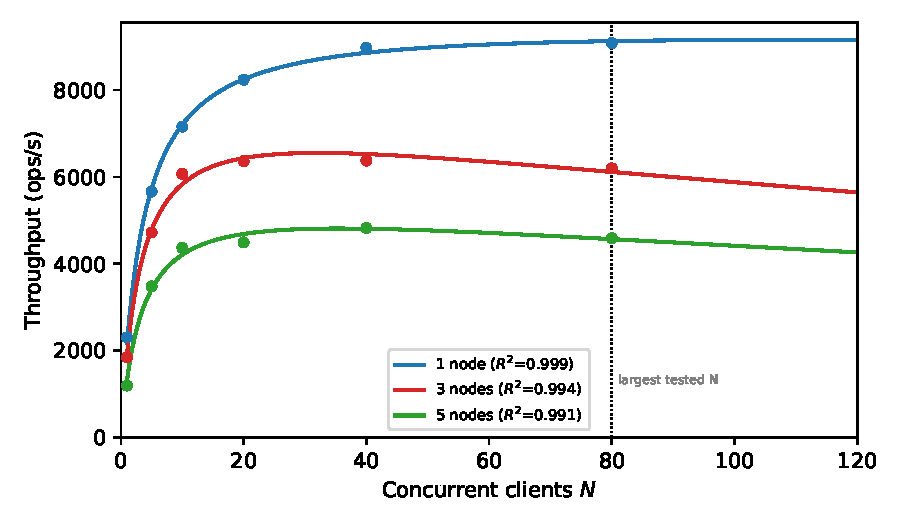
\includegraphics[width=0.75\textwidth]{usl_java_fit.pdf}
  \caption{Measured throughput and USL fits for 1, 3 and 5 servers (30\%
    writes). The curves are extended past the largest tested concurrency
    (80 clients) to show the predicted peaks.}
  \label{fig:usl}
\end{figure}

\paragraph{Three readings of the table.}
First, \textbf{$\alpha$ is stable at 0.22--0.24 across ensemble sizes}; the
three estimates overlap within their standard errors. Second,
\textbf{$\gamma$ falls as servers are added} (2174, 1907, 1329 ops/s), and
so does the measured single-client throughput (2302, 1839, 1191). The
single-client latencies from the raw data show where this comes from: the
median write latency at one client rises from 0.55\,ms (1 server) to
0.83\,ms (3) and 1.41\,ms (5), while the median read latency moves much
less (0.33, 0.38, 0.48\,ms). This is the expected per-write cost of the
proposal/ACK round trips and per-follower \texttt{fsync} in Zab, and it
is consistent with the read/write asymmetry we hypothesized. Third,
\textbf{$\beta$ is small but nonzero at 3 and 5 servers} ($7.3$ and
$6.0\times10^{-4}$, i.e.\ about 4 and 2.7 standard errors from zero), while at one
server it is indistinguishable from zero ($6.2\times10^{-5}$ with an error
larger than the estimate). With $\beta\approx0$ the standalone server is
classified as contention-bound, with a plateau and no predicted
decline. With $\beta>0$, the 3- and 5-server ensembles are predicted to peak near
$N_{\max}\approx32$--36 clients and then decline.

\paragraph{How strong is the retrograde effect?} The measured data support
the direction of the prediction but only weakly. At 3 servers throughput is
flat from 20 to 40 clients (6364, 6373) and then 2.8\% lower at 80 (6197);
at 5 servers it peaks at 40 (4824) and is 4.9\% lower at 80 (4588). Each
ensemble has a single point beyond its predicted peak, and the 3-server
20-to-40 plateau is within run-to-run noise, so we regard retrograde
behavior as supported but not conclusively demonstrated. Establishing it
would need concurrency levels beyond 80 and repeated runs.

\subsection{Interpreting $\alpha$: server-side, but not Zab-specific}

The straightforward hypothesis was that $\alpha\approx0.23$ reflects Zab's
strict leader serialization. But the standalone server has no leader, no
proposals and no quorum, and its fitted $\alpha$ (0.224) is the same as the
replicated ensembles' within error. So the serialization that dominates
at this scale is present in a single ZooKeeper server and is not introduced
by Zab. The most plausible source is the server's own request
pipeline, which processes requests through single-threaded stages
(request preparation, a log-sync stage that batches \texttt{fsync}s, and a
final commit/apply stage), together with the shared host disk. The server
metrics agree with a queue forming at the single server: the mean number of
outstanding requests on the standalone server grows from 0.2 at one client
to about 3.9 at 80 clients (with a maximum sample of 36), while the
leader's outstanding-request queue in the 3- and 5-server runs stays short
(mean below 1.2 at any concurrency). We sample this counter only at about
1\,Hz, so we treat it as supporting evidence, not proof.

Zab's costs therefore show up in the parameters that \emph{do} change with
ensemble size: $\gamma$ falls because each write pays for a quorum round
trip and follower \texttt{fsync}, and $\beta$ becomes measurable because
of the pairwise coordination that quorum acknowledgment requires. We did not
isolate the fsync, network and CPU components of these costs, and our
load generator and all servers share one host, so client-side CPU competition
is reduced but not excluded as a contributor to $\alpha$.

\subsection{Cross-validation against YCSB}

Table~\ref{tab:ycsb} gives the YCSB throughput on the 3-node ensemble.
Average update latency at 16 threads was 3713\,$\mu$s (A) and 2700\,$\mu$s
(B), against read latencies of 1078 and 831\,$\mu$s.

\begin{table}[h]
  \centering
  \caption{YCSB throughput (ops/s) by workload and thread count, 3-node
    ensemble.}
  \label{tab:ycsb}
  \begin{tabular}{@{}lrrrr@{}}
    \toprule
    Workload & 1 thread & 4 & 16 & 32 \\
    \midrule
    A (50/50 read/update) & 790  & 1316 & 1723  & 5964 \\
    B (95/5)              & 3544 & 6927 & 11436 & 8080 \\
    C (100\% read)        & 4538 & 9074 & 11913 & 8900 \\
    \bottomrule
  \end{tabular}
\end{table}

YCSB independently supports the main findings. Write-inclusive load costs
more: at 16 threads workloads C and B sustain 6.9$\times$ and 6.6$\times$
the throughput of the 50/50 workload A, and update latency is 3--4.5$\times$
read latency across both mixed workloads. This gap is consistent with the
write path's extra steps, though we did not instrument disk-sync time
separately from leader-forward and ACK time. Workloads B and C peak at 16
threads and then decline at 32 (11436$\to$8080; 11913$\to$8900), the same
retrograde direction as our fits for replicated ensembles. The absolute
numbers are of the same order as ours but not directly comparable, since the
write ratios differ (0\%, 5\% and 50\% against our 30\%).

We flag one anomaly rather than explain it away: workload A's throughput
jumps $3.5\times$ from 16 to 32 threads (1723$\to$5964) instead of
plateauing. We have no instrumented explanation (fixed operation count spread
across more threads, JVM warm-up or GC variance on a single non-repeated run
are candidates) and draw no conclusion from that point.

\subsection{Network chaos (extra credit)}

To see how the model behaves under a large per-request service-time
increase, we injected a 20\,ms egress delay with Pumba~\cite{pumba} (which
drives \texttt{tc netem}) into the container network namespaces of a 3-node
ensemble and re-ran the sweep. Single-client throughput $\gamma$ collapsed by
roughly $27\times$, as every operation that crosses a delayed link now pays
tens of milliseconds instead of well under one. Paradoxically, the fitted
$\alpha$ and $\beta$ dropped to near zero, and throughput scaled almost
linearly with clients up to 80.

This does not mean the delay removed the serialization or coherency cost. With
each client spending nearly all its time waiting on the injected delay, many
requests are in flight at once (pipelining), and the server-side stages
that produce $\alpha$ and $\beta$ are almost never busy at the same moment,
so no queue forms. The delay moves the saturation point far to the right of
the concurrency range we tested; it does not remove it. The
lesson for the USL is that $\alpha$ and $\beta$ describe behavior in the
regime measured and are not architecture constants: a fit that reports
near-zero contention is a statement about how far the system was pushed, and it
must be paired with the $\gamma$ collapse to be read correctly. Together with
the failover result (Section~\ref{sec:failover}), this shows that
the ensemble's throughput degrades sharply under network latency, and that
its availability under a node failure is good.

\section{Conclusion}

Fitting the USL to the sweep gives $R^2\ge0.99$ at every ensemble size and a
clear picture: contention $\alpha\approx0.23$ that does not depend on
ensemble size, an ideal throughput $\gamma$ that falls as servers are added
(2174$\to$1907$\to$1329 ops/s), and a small coherency term
$\beta\approx6$--$7\times10^{-4}$ that predicts a mild retrograde peak near
32--36 clients for 3 and 5 servers. The measured data show the decline only
at the 80-client point, so we report retrograde scaling as supported by the
fits and weakly observed.

The main analytical result is about where the costs sit. $\alpha$ is
present even on a standalone server, so we attribute it to ZooKeeper's
serialized request pipeline and shared host resources, not to Zab's leader
serialization; Zab's cost appears instead in $\gamma$ (each write pays a
quorum round trip and follower \texttt{fsync}) and in $\beta$. YCSB, an
independent load generator, reproduces the read/write cost asymmetry and the
peak-then-decline shape. A leader failover took 211\,ms of election time, and
a 20\,ms network delay cut $\gamma$ by roughly 27$\times$ while making the
fit look contention-free, a reminder that $\alpha$ and $\beta$ describe the
regime that was measured.

Limitations are the single-host deployment, the sweep ending at 80 clients,
one run per grid point, and the coarse 1\,Hz server metrics. For Stage II's
multi-machine deployment we would add repeated runs, concurrency beyond 80,
larger ensembles (7, 9), an fsync/network/CPU breakdown to locate the source
of $\alpha$, and an end-to-end measurement of client-observed failover.

\begin{thebibliography}{4}

\bibitem{apache_zookeeper_overview}
Apache Software Foundation.
\newblock ZooKeeper: A Distributed Coordination Service for Distributed
  Applications.
\newblock ZooKeeper 3.9.6 documentation, 2024.
\newblock \url{https://zookeeper.apache.org/doc/r3.9.6/zookeeperOver.html}.

\bibitem{mit_6824_zookeeper}
MIT 6.824: Distributed Systems.
\newblock ZooKeeper.
\newblock Lecture 8, Spring 2020.
\newblock \url{https://www.youtube.com/watch?v=pbmyrNjzdDk}.

\bibitem{gunther_usl_dsconf}
Distributed Systems Conference.
\newblock Applying The Universal Scalability Law to Distributed Systems by Dr. Neil J. Gunther.
\newblock DSConf 2019, March 16, 2019.
\newblock \url{https://www.youtube.com/watch?v=cuieNj3NrZ8}.

\bibitem{pumba}
A.~Ledenev.
\newblock Pumba: chaos testing and network emulation for Docker containers.
\newblock \url{https://github.com/alexei-led/pumba}.

\end{thebibliography}
\end{document}
